\documentclass[a4paper,12pt,twoside]{article}
\usepackage[polish]{babel}

\addto\captionspolish{\renewcommand{\figurename}{Rys.}}
\usepackage[utf8]{inputenc}
\usepackage[english]{babel}
\usepackage[margin=2cm]{geometry}
\usepackage[table,xcdraw]{xcolor}
\usepackage{graphicx}
\usepackage{indentfirst}
\usepackage{multicol}
\usepackage{listings}
\usepackage[T1]{fontenc}
\usepackage{bigfoot} % to allow verbatim in footnote
\usepackage[numbered,framed]{matlab-prettifier}
\usepackage{filecontents}
\usepackage{blindtext}
\usepackage{graphics}
\usepackage{adjustbox}
\usepackage{float}
\usepackage{subfigure}
\usepackage{multirow}
\usepackage{colortbl}
\usepackage{anyfontsize}
\usepackage{t1enc}
\usepackage{enumitem}
\usepackage{hhline}
\usepackage{fancyhdr}
\usepackage{marginnote}
\usepackage{amsmath}
\usepackage{amsthm}
\usepackage{mathtools}
\usepackage{dirtytalk}
\usepackage{cite}
\usepackage[font=footnotesize, labelfont=bf]{caption}
\usepackage{textgreek} %for units like micro in text
\usepackage[hidelinks]{hyperref}
\usepackage{adjustbox}
\urlstyle{same}
\usepackage{physics}
\usepackage{chemfig}
\renewcommand{\figurename}{Rys.}
\title{\textbf{Projekt 4: Proste całkownie z szacowaniem wariancji.}}
\author{Kacper Połuszejko, 412183}
\date{}
\begin{document}
\maketitle

\section*{Wstęp}

Celem ćwiczenia było oszacowanie powierzchni części wspólnej dwóch kół metodą całkowania Monte Carlo. \\

Koła na płaszczyźnie definiujemy w następujący sposób:

\begin{equation}
K_A = \left\{ (x, y) : (x - x_A)^2 + (y - y_A)^2 \leq R_A^2 \right\}
\end{equation}

\begin{equation}
K_B = \left\{ (x, y) : (x - x_B)^2 + (y - y_B)^2 \leq R_B^2 \right\}
\end{equation}

\section{Metodyka}

\subsection{Generator rozkładu jednorodnego w kole}

Do wygenerowania punktów w danym kole wykorzystujemy rozkład jednorodny sferycznie konturowany. Losowanie przeprowadzamy na podstawie poniższego algorytmu.

\begin{equation*}
\begin{aligned}
u_1, u_2 &\sim U(0,1) \\
x &= \sqrt{-2\ln(u_1)}\sin(2\pi u_2) \\
y &= \sqrt{-2\ln(u_1)}\cos(2\pi u_2) \\
r &= \sqrt{x^2 + y^2} \\
x &\leftarrow \frac{x}{r} \\
y &\leftarrow \frac{y}{r}
\end{aligned}
\end{equation*}

\begin{equation*}
\begin{aligned}
u_3 &\sim U(0,1) \\
q &= \sqrt{u_3} \\
x &\leftarrow q \cdot x \cdot R_\alpha + x_\alpha \\
y &\leftarrow q \cdot y \cdot R_\alpha + y_\alpha
\end{aligned}
\end{equation*}

\subsection{Powierzchnia części wspólnej}


Powierzchnię koła znajdziemy licząc całkę po powierzchni koła \( K_\alpha \)
\begin{equation}
S_\alpha = \iint\limits_{(x,y)\in K_\alpha} 1 \, dx\,dy = \iint\limits_{(x,y)\in K_\alpha} \frac{1}{f_\alpha(x,y)} f_\alpha(x,y)\,dx\,dy = \pi R_\alpha^2 \iint\limits_{(x,y)\in K_\alpha} f_\alpha(x,y)\,dx\,dy,
\end{equation}
 gdzie $f_\alpha(x,y) = const = C = \frac{1}{\pi R^2_{\alpha}}$ jest fgp rozkładu jednorodnego w kole. \\


Analogicznie możemy zdefiniować całkę powierzchniową dla części wspólnej
\begin{equation}
S_{\alpha,\beta} = \pi R_\alpha^2 \iint\limits_{(x,y)\in K_\alpha} \theta_{\alpha,\beta}(x,y)\,dx\,dy
\end{equation}

\begin{equation}
\theta_{\alpha,\beta}(x,y) = 
\begin{cases}
1 &\Leftrightarrow (x,y) \in K_\alpha \wedge (x,y) \in K_\beta \\
0 & \text{w przeciwnym wypadku}
\end{cases}
\end{equation}

\(\theta\) pełni rolę funkcji wskaźnikowej o wartości binarnej (metoda eliminacji). Pole powierzchni części wspólnej w MC liczymy jako średnią z \(N\) wartości funkcji podcałkowej (\(\mu^{(1)}\) - pierwszy moment rozkładu)
\begin{equation}
\mu^{(1)} = \bar{S}_{\alpha,\beta} = \frac{1}{N} \sum_{i=1}^N \pi R_\alpha^2 \theta_{\alpha,\beta}(x_i,y_i)
\end{equation}

gdzie punkty \((x_i, y_i)\) losujemy z rozkładu jednorodnego w kole \(K_\alpha\). Analogicznie liczymy drugi moment, uwzględniając własność \(\theta_{\alpha,\beta}^2 = \theta_{\alpha,\beta}\)
\begin{equation}
\mu^{(2)} = \frac{1}{N} \sum_{i=1}^N \left( \pi R_\alpha^2 \theta_{\alpha,\beta}(x_i,y_i) \right)^2 = \pi R_\alpha^2 \left( \frac{1}{N} \sum_{i=1}^N \pi R_\alpha^2 \theta_{\alpha,\beta}(x_i,y_i) \right) = \pi R_\alpha^2 \mu^{(1)}
\end{equation}

Mając pierwszy i drugi moment możemy policzyć wariację wartości średniej
\begin{equation}
\sigma_{S_{\alpha,\beta}}^2 = \frac{\mu^{(2)} - \left(\mu^{(1)}\right)^2}{N}
\end{equation}

i odchylenie standardowe wartości średniej
\begin{equation}
\sigma_{S_{\alpha,\beta}} = \sqrt{ \frac{ \mu^{(2)} - \left( \mu^{(1)} \right)^2 }{N} }
\end{equation}

\newpage

\section{Wyniki}
W obliczeniach przyjęto parametry:

$R_A = 2, R_B = \sqrt{2}R_A, \vec{r_A} = [x_a, 0], \vec{r_B} = [0, 0]$. 

\subsection{Test generatora}

Przeprowadzono test generatora przyjmując parametry $x_a = R_a + R_b$ oraz $N = 10^4$. 

\begin{figure}[h!]
    \centering
    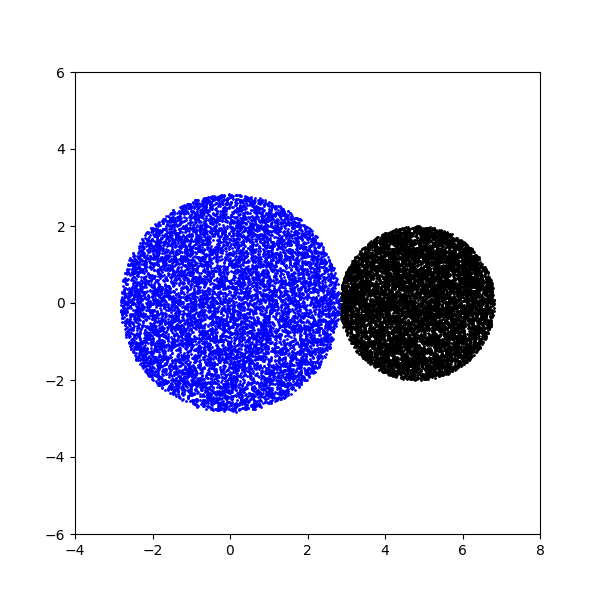
\includegraphics[width=0.65\linewidth]{Carlo_4_1.png}
    \caption{Rozkład jednorodny w kole $K_A$ oraz $K_B$.}
\end{figure}

Jak widać na powyższym rysunku, wyniki zgadzają się z przewidywaniami, generatory działają więc poprawnie.

\subsection{Pole powierzchni części wspólnej}
Na podstawie wzorów (6) oraz (9) obliczono średnią oraz jej odchylenie standardowe dla czterech przypadków ($N = 10^6$):

\begin{enumerate}
  \item[a)] $\alpha = A,\ x_A = R_B + 0.5 \cdot R_A$
  \item[b)] $\alpha = A,\ x_A = 0$
  \item[c)] $\alpha = B,\ x_A = R_B + 0.5 \cdot R_A$
  \item[d)] $\alpha = B,\ x_A = 0$
\end{enumerate}
\newpage
Otrzymane wyniki:

 \begin{figure}[h!]
    \begin{minipage}{0.55\textwidth}
        \centering
        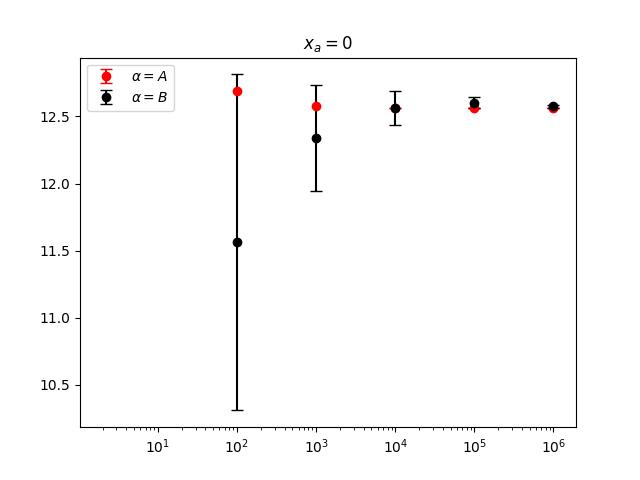
\includegraphics[scale = 0.5]{Carlo_4_2.jpg}
    \end{minipage}
    %\hspace{15mm}
    \begin{minipage}{0.55\textwidth}
        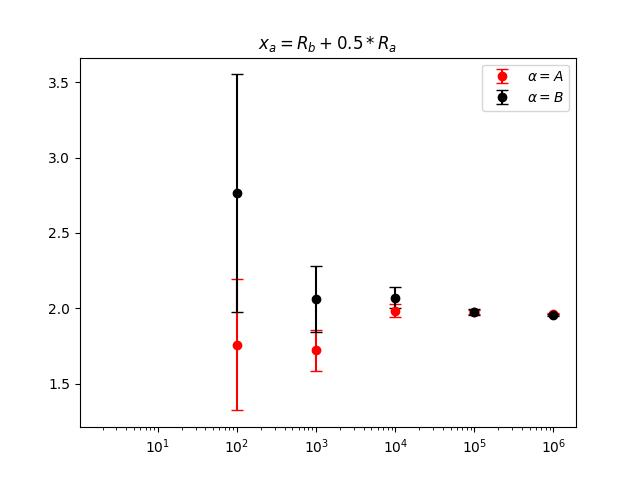
\includegraphics[scale = 0.5]{Carlo_4_3.jpg}
    \end{minipage}
    \caption{Wspołna powierzchnia dla całkowitego (po lewej) i częściowego nakładanie się kół (po prawej).  }
\end{figure}

Jak widać na powyższych wykresach, średnia z N wartości funkcji podcałkowej zbiega się do pewnej wartości, natomiast odchylenie standardowe maleje. Jest to zgodne z przewidywaniami oraz prawem wielkich liczb. Warto zauważyć, że dla $x_a = 0, \alpha = A$ odchylenie standardowe jest bliskie zeru. Jest to spowodowane faktem, że dla tak przyjętego $x_a$ koło $K_A$ całkowicie zawiera się w $K_B$. Wykonując więc całkowanie Monte Carlo na podstawie rozkładu jednorodnego w $K_A$ każdy losowany punkt zawiera się w obu kołach i funkcja (5) jest zawsze równa jeden. 

\end{document}
